\begin{figure}[htbp]
	\centering
	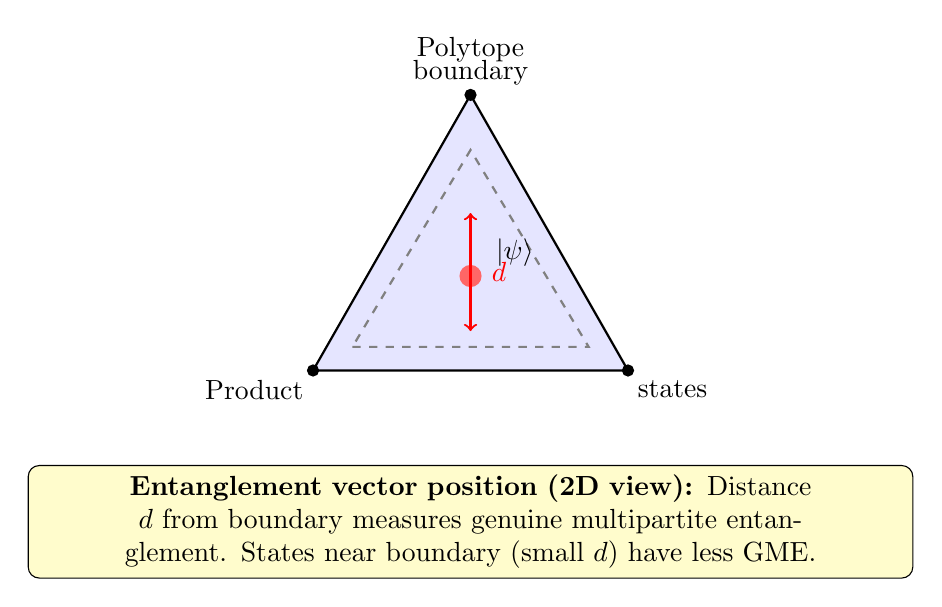
\begin{tikzpicture}[scale=1.0]
		\draw[thick, fill=blue!10] (0,0) -- (4,0) -- (2,3.5) -- cycle;
		\draw[dashed, thick, gray] (0.5,0.3) -- (3.5,0.3) -- (2,2.8) -- cycle;

		\fill[red!60] (2,1.2) circle (4pt);
		\node[above right] at (2.2,1.2) {$|\psi\rangle$};

		\draw[fill=black] (0,0) circle (2pt);
		\draw[fill=black] (4,0) circle (2pt);
		\draw[fill=black] (2,3.5) circle (2pt);

		\node[below left] at (0,0) {Product};
		\node[below right] at (4,0) {states};
		\node[above] at (2,3.8) {Polytope};
		\node[above] at (2,3.5) {boundary};

		\draw[<->, thick, red] (2,0.5) -- (2,2) node[midway, right=4pt] {$d$};

		\node[draw, rounded corners, fill=yellow!20, text width=11cm, align=center, below=0.8cm] at (2,-0.4) {
			\textbf{Entanglement vector position (2D view):} Distance $d$ from boundary measures genuine multipartite entanglement. States near boundary (small $d$) have less GME.
		};
	\end{tikzpicture}
	\caption{Entanglement polytope showing the position of a state $|\psi\rangle$ within the polytope (2D projection). The distance $d$ from the boundary indicates the amount of genuine multipartite entanglement.}
	\label{fig:entanglement-polytope-position-2d}
\end{figure}
